\chapter{Methodology}

% \section{Research Methodology}
% \label{introduction:research-methodology}

\noindent
To achieve the main goal of the thesis and answer the identified research questions,
a mix of different scientific methods is used.
The primary method for creating empirical value - design and development of a software prototype - is the prototyping method as described by
\citeauthor{riedlManagementInformatik2019} (\citeyear{riedlManagementInformatik2019}).
It is supported, especially for defining and motivating the problem statement, by
semi-structured qualitative interviews according to the method of \autocite{glaser2010experteninterviews}.
%
In order to help with recognition and legitimization of the conducted research,
the methodology for conducting design science (DS) research
in information systems (IS)
\autocite{designScienceResearchMethodologyForInformationSystemsResearch}
is applied.
It consists of six activities:
Activity 1: Identify Problem \& Motivate;
Activity 2: Define Objectives of a Solution;
Activity 3: Design \& Development;
Activity 4: Demonstration;
Activity 5: Evaluation;
Activity 6: Communication.
%
%\begin{itemize}
%	\item Activity 1: Identify Problem \& Motivate
%	\item Activity 2: Define Objectives of a Solution
%	\item Activity 3: Design \& Development
%	\item Activity 4: Demonstration
%	\item Activity 5: Evaluation
%	\item Activity 6: Communication
%\end{itemize}
%
The process is structured in a nominally sequential order.
For this concrete research,
the problem-centered initiation is chosen as the entry point,
thus the process will begin with activity 1.
Afterwards the research will proceed sequentially,
because the idea of the research resulted from observation of the problem
\autocite{designScienceResearchMethodologyForInformationSystemsResearch}.

In activity 1,
the research problem of
release promotion with GitOps
is defined.
This is accomplished, by
seeking knowledge of the state of the problem
from practicing professionals.
This is done by conducting
semi-structured interviews,
%, as described in section \ref{methodology:interview},
as well as analysing prior written literature.
To assist later evaluation,
the problem is conceptually broken down into distinct items.
%(fig. \ref{fig:problemToObjectiveMapping}).
%
%\begin{figure}[h]
%	\centering
%	\fbox{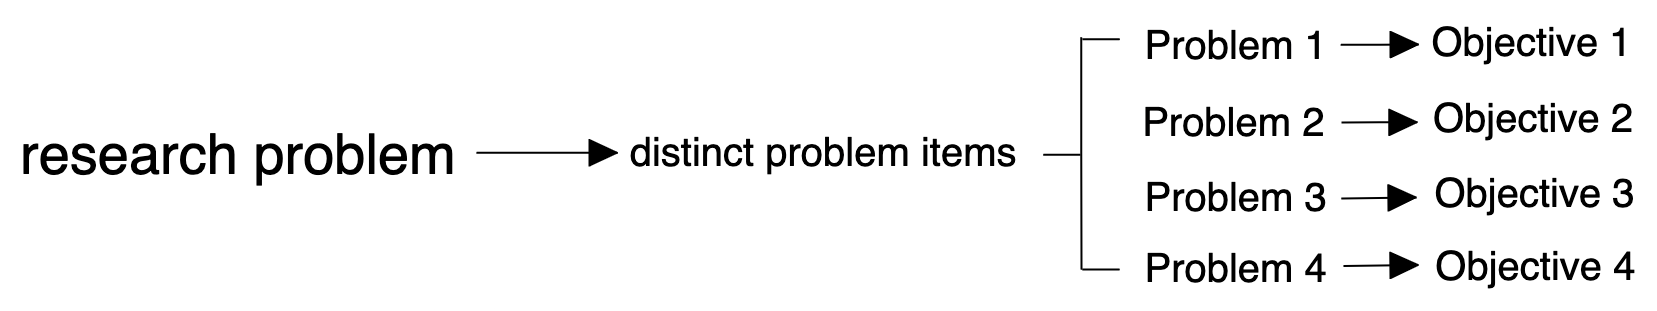
\includegraphics[width=0.85\linewidth]{assets/problem-to-objective-mapping.png}}
%	\caption{Inference of objectives from problems.
%		%		(\citeauthor{ref}, \citeyear{ref}).
%	}
%	\label{fig:problemToObjectiveMapping}	
%\end{figure}
%
The value of a solution is highlighted,
in order to help the audience of the research
understand the reasoning associated with the
researcher's understanding of the problem
\autocite{designScienceResearchMethodologyForInformationSystemsResearch}.
%
In activity 2,
research objectives are inferred from the problem definition in activity 1.
Each objective maps to a distinct item from the problem specification,
%(illustrated in Figure \ref{fig:problemToObjectiveMapping}),
which helps with later evaluation in activity 5.
In practice, a research objective is a qualitative description of
how a new artifact is expected to support a solution to the problem definition.
%
In activity 3,
solutions for the previously defined objectives are designed and developed
by means of producing an artifact.
This is achieved by
determining the artifact's desired functionality and its architecture,
followed by actually creating the artifact
\autocite{designScienceResearchMethodologyForInformationSystemsResearch}.
In practice this means that:
Abstract model definitions are designed;
with the specification of the model definitions in place,
the \textit{GitOps Promotions Operator} prototype is developed as an artifact.
%
In activity 4,
the in-context use of the artifact is demonstrated in a proof of concept.
The prototype operator is used in a practical use case of a promotion in a GitOps environment.
A description of the setup, the use and observed functionality is demonstrated.
%
In activity 5,
the implementation of the artifact,
and how well it supports a solution to the problem,
is evaluated.
This is achieved by
comparing the objectives of a solution to actual observed results
from use of the artifact in the demonstration
\autocite{designScienceResearchMethodologyForInformationSystemsResearch}.
In practice this means, that
the functionality of the artifact implemented in the prototype in activity 4,
is compared with the solution objectives from activity 2.
%
In activity 6, as a final step,
the whole conducted research is communicated by means of
disclosing
the problem and its importance,
the artifact and its utility and novelty,
and the demonstration accompanied by the evalution results
\autocite{designScienceResearchMethodologyForInformationSystemsResearch},
within the publication of a master thesis at
the University of Applied Sciences Burgenland
%\footnote{https://www.fh-burgenland.at/}.
In addition, it is communicated to relevant audiences such as
the GitOps Working Group
%\footnote{https://github.com/cncf/tag-app-delivery/tree/main/gitops-wg}
of the CNCF.




















%existing literature on the topic is analysed,
%in order to find out 
%what current best practices and tools
%which address the given problem
%are already available within the open-source community.
%Second,
%
%In the beginning, existing literature on the topic, 
%as well as the concrete research questions
%are discussed.
%Furthermore, various
%opinions and approaches of pioneering organizations in the GitOps community
%are analyzed.
%% how? What exactly are you analyzing?
%\bigskip
%
%\noindent
%Next, existing software solutions,
%which are available under open source licenses,
%will be evaluated for their appropriate use for the present research.
%The aim is to find out the extent to which the defined research questions
%can be addressed with existing solutions.
%Finally, a baseline is defined as state-of-the-art.
%\bigskip
%
%\noindent
%Furthermore, abstract models for deployment environments
%and promotion workflows will be defined.
%These serve as a basis for the design of the prototype in the next step.
%\bigskip
%
%\noindent
%As far as possible and reasonable, existing toolkits and best practices will be used for the prototype.
%It is desirable to solely extend
%the Kubernetes-API
%% cite
%and the
%GitOps-Toolkit
%% cite
%to integrate the prototype natively into the existing ecosystem around GitOps within the CNCF.
%\bigskip
%
%\noindent
%According to 
%\citeauthor{HOUDE1997367} (\citeyear{HOUDE1997367})
%a prototype is any representation of a design idea, regardless of the medium.
%A prototype is something that serves as a model or inspiration for later developments
%\autocite{HOUDE1997367}.
%\bigskip
%
%\noindent
%The developed prototype will be compared to existing approaches to solving the problem in a laboratory experiment.
%\bigskip
%
%\noindent
%\citeauthor{montgomery2017design} (\citeyear{montgomery2017design})
%defines an experiment as a test 
%or series of runs in which intentional changes are made to the input variables, 
%in order to then observe and identify reasons for changes in the output result
%\autocite{montgomery2017design}.

%Nach erfolgreicher Implementierung des Prototyps,
%soll mittels einer Scheduler-Extension in einem Laborexperiment gezeigt werden,
%dass Kubernetes Workloads adaptiv Nodes zugeordnet werden können,
%auf welchen diese die beste Energieeffizienz aufweisen.
%\bigskip

%Das Ziel dabei ist etwas Neues bei einem System oder Prozess zu entdecken, 
%oder eine bestehende Theorie zu beweisen
%\autocite{montgomery2017design}.
%\bigskip




